%% Journal of Open Research Software Latex template - Created By Stephen Bonner and John Brennan, Durham Universtiy, UK.
%% REVISED VERSION — addresses reviewer comments R1–R7
%% Placeholders to fill before submission:
%%   [ZENODO DOI]           — Zenodo persistent identifier (deposited 15 Apr 2026)
%%   [COMMERCIAL SOFTWARE]  — name and version of commercial FEM tool used in Fig. 2 validation

\documentclass{jors}
\usepackage{graphicx}
\usepackage{booktabs}

%% Set the header information
\pagestyle{fancy}
\definecolor{mygray}{gray}{0.6}
\renewcommand\headrule{}
\rhead{\footnotesize 3}
\rhead{\textcolor{gray}{UP JORS software Latex paper template version 0.1}}

\begin{document}

{\bf {pyCAFE: A Finite Element Framework for Solving Acoustic Problems in Python}} \\ \\

Please submit the completed paper to: editor.jors@ubiquitypress.com

\rule{\textwidth}{1pt}

\section*{(1) Overview}

\vspace{0.5cm}

\section*{Title}

pyCAFE: A Finite Element Framework for Solving Acoustic Problems in Python

\section*{Paper Authors}

1. Fabbri, Daniele; (Lead/corresponding author first) \\
2. Bruzzone, Fabio; 3. Rosso, Carlo

\section*{Paper Author Roles and Affiliations}
1. Fabbri, Daniele; Conceptualization, software development, numerical implementation, validation, and manuscript preparation. Affiliation: Department of Mechanical and Aerospace Engineering, Politecnico di Torino, Turin, Italy.\\
2. Supervision, and critical review of the manuscript. Affiliation: Department of Mechanical and Aerospace Engineering, Politecnico di Torino, Turin, Italy.\\
3. Supervision, and critical review of the manuscript. Affiliation: Department of Mechanical and Aerospace Engineering, Politecnico di Torino, Turin, Italy.

\section*{Abstract}

pyCAFE is an open-source Python framework for the numerical solution of two-dimensional, frequency-domain acoustic problems governed by the Helmholtz equation using the Finite Element Method. The software implements explicit assembly of global acoustic stiffness and mass matrices from element-level contributions using bilinear four-node (CQUAD4) and serendipity eight-node (CQUAD8) quadrilateral elements. It supports prescribed pressure, prescribed normal velocity, impedance, and rigid boundary conditions, and provides both direct frequency-domain solvers and a modal solver based on a sparse generalised eigenvalue problem. pyCAFE operates on two-dimensional meshes generated with Gmsh and follows a matrix-based workflow conceptually aligned with commercial finite element software, exposing the discretised system operators directly to the user. The framework includes an automated test suite covering element-level properties, boundary condition enforcement, and solver accuracy, together with a GitHub Actions continuous integration pipeline verified on Python 3.10--3.12. Analytical validation against closed-form eigenfrequencies for a rigid rectangular cavity demonstrates relative errors below $0.001\,\%$ for CQUAD8 discretisations. Originally developed as a MATLAB code, the framework has been ported to Python to improve accessibility and integration with open scientific libraries for research and teaching in computational acoustics.

\section*{Keywords}

Acoustics; Finite Element Method; Python; Helmholtz equation; frequency domain; modal analysis; CQUAD8; computational acoustics; open source

\section*{Introduction}

Computational acoustics plays a central role in the numerical analysis of sound propagation in enclosed and semi-enclosed domains, such as ducts, cavities, and waveguides. In these applications, frequency-domain formulations are widely adopted, particularly when time-harmonic responses are of interest. For complex geometries and boundary conditions, analytical solutions are generally not available, making numerical approaches essential. Among the available numerical methods, the Finite Element Method (FEM) is commonly employed due to its ability to discretize arbitrary geometries and to systematically incorporate a wide range of acoustic boundary conditions. The theoretical foundations of finite element formulations for acoustic problems are well established and extensively documented in the literature \cite{MacNeal1994,Desmet1999,Ihlenburg1995,Babuska1988,Prinn2023}, building on general numerical concepts originally developed for structural mechanics and later extended to acoustics. Solving the acoustic field in enclosed and open domains is widely used in both academia and industry \cite{HelmholtzResonator2012,Thompson2006,Harari2006,Khalefa2024}. This work focuses on low-to-mid frequency analyses, broadly understood here as the regime where the acoustic wavelength is at least two to three times the element size so that polynomial interpolation is accurate; in practice this corresponds to a maximum non-dimensional wave number $kh < 1$ on the mesh, where $k = \omega/c_0$ is the wave number and $h$ is the characteristic element size. While some open-source tools can solve Helmholtz-type problems, many frameworks adopt a variational weak-form workflow in which the governing equations are expressed symbolically and assembled implicitly. In contrast, open-source software adopting a matrix-based finite element approach aligned with common commercial FEM practice remains limited. In such an approach, element-level contributions are assembled explicitly into global system matrices and boundary operators are handled transparently. This design emphasises numerical clarity, reproducibility, and direct inspection of the discretised operators, facilitating validation and benchmarking.

Several open-source alternatives exist for frequency-domain acoustic and general PDE simulation. FEniCSx \cite{FEniCSx2023} is a general-purpose problem-solving environment based on the Unified Form Language; it supports a broad class of PDEs through variational formulations but does not expose the assembled system matrices directly in the workflow. FreeFEM \cite{Hecht2012} offers a scripting-based approach for FEM on unstructured meshes but is not Python-native. scikit-fem \cite{skfem2020} provides lightweight sparse-matrix assembly in Python for general elliptic problems. openCFS \cite{openCFS2022} targets coupled field simulations including acoustics but requires a dedicated mesh and solver pipeline. These frameworks differ from pyCAFE in scope and design philosophy: pyCAFE deliberately targets the two-dimensional acoustic Helmholtz problem with a matrix-based assembly that mirrors the workflow of commercial FEM codes, providing users with direct access to the stiffness and mass operators, explicit boundary condition matrices, and a modal solver suited for educational and validation-oriented use. The MATLAB predecessor CAFE \cite{Fabbri2025} established this design philosophy; the present Python port extends accessibility while preserving numerical transparency.

From a numerical discretisation perspective, the same matrix-based strategies used for structural discretisation can be applied to the acoustic domain, leading to stiffness, mass, and damping-based formulations that also form the basis for vibroacoustic coupling \cite{Nefske1976,Beriot2021}. Subsequent developments showed that structural and acoustic domains may be assembled into a unified coupled system, enabling eigenvalue or time-harmonic analyses when required. While such coupled formulations and additional techniques such as absorbing domains \cite{Turkel1998,Pekel1995,Reheman2013} represent important extensions of acoustic FEM, the present work focuses exclusively on the two-dimensional acoustic domain, building upon this established theoretical foundation.

CAFE (Computational Acoustic Finite Elements) \cite{Fabbri2025} was originally developed as an open-source MATLAB framework to address this gap by providing a clear and accessible implementation of frequency-domain acoustics. The present work introduces pyCAFE, the Python translation of the original framework. The port to Python was motivated by the desire to improve accessibility and integration with modern open scientific libraries, while preserving the numerical philosophy and workflow of the original code. The software is available at \url{https://github.com/DanFabb/pycafe} and can be installed via \texttt{pip install pycafe}. A persistent software archive is available at \url{https://doi.org/[ZENODO DOI]}.

The software was designed to explicitly assemble acoustic stiffness, mass, and damping matrices while following a modelling workflow conceptually aligned with that of commercial finite element software. This design choice facilitates validation, benchmarking, and educational use by exposing the numerical operators involved in the discretised problem. pyCAFE operates on externally generated two-dimensional finite element meshes, typically produced using Gmsh \cite{Gmsh2009}, and supports commonly used boundary conditions in frequency-domain acoustics.

\section*{Implementation and architecture}

The pyCAFE architecture is structured around a folder called \textit{core} that oversees the simulation workflow and delegates particular duties to a group of modular subfolders. Figure \ref{Fig1} depicts a schematic overview of the software architecture.
\begin{figure}[h]
    \centering
    \includegraphics[width=0.8\linewidth]{1.jpg}
    \caption{Overall architecture of the pyCAFE framework and main software modules.}
    \label{Fig1}
\end{figure}
The workflow is structured by using Python scripts that import the submodules instead of embedding problem logic in the core. This design choice was deliberately chosen to allow users to define simulation parameters, boundary conditions, and analysis options directly via keyboard input, without modifying the core implementation. By separating user-driven input and problem configuration from the numerical backend, pyCAFE offers a flexible interface for custom simulations while keeping the core solver stable and intact. Mesh generation and geometry definition are handled externally. pyCAFE assumes that geometries are created following a predefined syntax compatible with Gmsh input files. The software provides auxiliary scripts for geometry creation to ensure consistent naming conventions and physical group definitions to support this process. A dedicated mesh loading module is used to import the mesh after it is generated. The material properties of the acoustic medium are defined separately, allowing users to specify fluid parameters independently of the mesh and geometry. Boundary conditions are assigned through a dedicated module that currently supports interactive input via the keyboard. This approach mirrors the conceptual workflow of commercial finite element software, where boundary conditions are explicitly defined and independent of the solver. The assembled acoustic system is passed to solver routines that support both direct frequency-domain solutions and modal-based approaches. Post-processing utilities are integrated at this stage to allow inspection and visualisation of acoustic pressure fields and derived quantities. The separation between solver logic and post-processing further enhances modularity and enables users to adapt or replace individual components according to their specific needs.

\subsection*{Geometry and material selection}
pyCAFE operates on externally generated two-dimensional meshes and provides helper scripts to understand how the geometry definition, meshing, and material parameter selection should be done to comply with the software. The geometry module currently supports the interactive creation of simple benchmark domains (rectangular and circular cavities) through keyboard input. Users specify the geometric parameters, the maximum frequency of interest, and the desired element order (linear or quadratic). Mesh generation is performed through the Gmsh Python API \cite{Gmsh2009}; in addition to creating the geometric entities, the script assigns physical groups to both the domain and each boundary segment. To facilitate reproducible workflows, the generated mesh is saved to a user-selected location via a file dialog. A companion mesh visualisation utility can then be used to load an existing \texttt{.msh} file, extract node coordinates, element connectivities, and physical boundary groups, and provide a quick 2D plot for inspection. Material properties for the acoustic medium are defined independently from the mesh. A dedicated material utility provides predefined parameter sets for common fluids (e.g., air and water) and supports custom user-defined media. For convenience, the characteristic impedance $Z_0 = \rho_0 c_0$ is computed and returned together with the selected density and sound speed, ensuring consistent parameter handling throughout the analysis pipeline.

\subsection*{Build matrices}
The \textit{build matrices} folder contains the numerical routines for the construction of the acoustic finite element operators. This module implements the element-level formulations required to assemble the global stiffness, mass, and damping matrices starting from the discretised mesh. Two quadrilateral element types are supported: the bilinear four-node element (CQUAD4) employing a $2 \times 2$ Gauss integration rule, and the serendipity eight-node quadratic element (CQUAD8) employing a $3 \times 3$ Gauss rule \cite{Beriot2016}. Each element type is defined in a dedicated module providing shape functions, Jacobian computation, and element matrix assembly. The element type is detected automatically from the imported mesh and the corresponding formulation is invoked transparently, removing the need for manual user intervention when switching between linear and quadratic discretisations. This separation ensures that element-level implementations are self-contained and can be individually unit-tested.

CQUAD4 elements yield an asymptotic eigenvalue convergence rate of $O(h^2)$ and CQUAD8 elements yield $O(h^4)$, consistent with standard FEM approximation theory for smooth solutions \cite{Ihlenburg1995,Babuska1988}. Both rates have been confirmed numerically via log-log regression on a rectangular cavity benchmark (see Section Quality Control). By following a fully matrix-based approach, the resulting operators are directly accessible to the user, enabling inspection, debugging, and validation against reference solutions.

\subsection*{Boundary condition assignment}
Boundary conditions in pyCAFE are assigned through a keyboard-driven terminal interface. Boundary identification relies on the physical groups defined in the Gmsh mesh; for each boundary detected in the mesh, the user is prompted to select the desired acoustic boundary condition via keyboard input. The assignment procedure is intentionally decoupled from the solver and matrix assembly routines, allowing boundary conditions to be modified without altering the core numerical implementation. The following acoustic boundary condition types are currently supported:
\begin{itemize}
    \item rigid (sound-hard) boundaries, which represent the default condition and enforce zero normal particle velocity;
    \item zero pressure boundaries, where the acoustic pressure is prescribed to vanish;
    \item constant pressure boundaries, in which a uniform pressure amplitude is imposed along the selected boundary;
    \item impedance boundaries, where a complex acoustic impedance relates pressure to normal velocity;
    \item prescribed normal velocity boundaries, typically used to model vibrating surfaces or velocity-driven acoustic excitation.
\end{itemize}
In addition to boundary-based conditions, the framework also supports localised acoustic excitation through a point pressure source. The user specifies the spatial coordinates of the source, and the closest mesh node is automatically identified and selected. A pressure amplitude is then assigned to this node and incorporated directly into the acoustic load vector. All boundary condition information is collected and returned in a structured data container, which is subsequently passed to the matrix assembly and solver routines.

\subsection*{Solver and post-processing}
Once the global acoustic system matrices have been assembled, pyCAFE provides both direct and modal solution strategies in the frequency domain. The user can explicitly select the preferred approach depending on the analysis objective.

In the direct solution strategy, the frequency-domain acoustic problem is solved independently at each frequency of interest. The treatment of boundary conditions distinguishes between two mathematically distinct types: natural (Neumann) conditions and essential (Dirichlet) conditions.

\textit{Natural boundary conditions} --- rigid walls, prescribed normal velocity, and impedance --- arise directly from the weak form of the Helmholtz equation and require no modification to the system matrices. Rigid walls correspond to the homogeneous Neumann condition $\partial p / \partial n = 0$ and are satisfied by default. Prescribed normal velocity $v_n$ contributes a frequency-dependent term $\mathrm{i}\,\omega\,\rho\,v_n \int_\Gamma N \, \mathrm{d}s$ to the right-hand-side vector, assembled using one-dimensional quadratic (Line3) boundary elements consistent with the CQUAD8 interior discretisation. Impedance boundaries add an admittance-weighted surface integral $\mathrm{i}\,\omega\,\rho\,Y \int_\Gamma N_i N_j \, \mathrm{d}s$ to the system, where $Y = 1 / (\zeta \rho c_0)$ is the specific acoustic admittance.

\textit{Essential boundary conditions} --- prescribed pressure --- must be imposed explicitly and are handled in two stages. In the first stage, boundaries with zero pressure ($p = 0$) are eliminated from the global system at assembly time: the rows and columns corresponding to those degrees of freedom are permanently removed from $\mathbf{K}$, $\mathbf{M}$, and $\mathbf{C}$, yielding reduced operators $\mathbf{K}_\mathrm{red}$, $\mathbf{M}_\mathrm{red}$, $\mathbf{C}_\mathrm{red}$ of smaller size. In the second stage, non-zero prescribed pressures are enforced at solve time via a partitioned formulation \cite{Guyan1965,Kidder1973}: the reduced system is further split into known degrees of freedom (those with prescribed $p = p_0$) and unknowns, and the linear system
\begin{equation}
  \mathbf{A}_{ii} \, \mathbf{p}_i = \mathbf{f}_i - \mathbf{A}_{in} \, \mathbf{p}_0
\end{equation}
is solved for the unknowns $\mathbf{p}_i$, where $\mathbf{A} = \mathbf{K}_\mathrm{red} + \mathrm{i}\,\omega\,\mathbf{C}_\mathrm{red} - \omega^2 \mathbf{M}_\mathrm{red}$. This is the standard static condensation approach; it is algebraically exact and introduces no approximation. Sparse direct solvers are employed when available \cite{Damhaug1993}.

In addition to the direct approach, pyCAFE includes a modal solver for acoustic analysis. The solver computes natural frequencies and corresponding acoustic mode shapes by solving the generalised symmetric eigenvalue problem $\mathbf{K}\boldsymbol{\phi} = \omega^2 \mathbf{M}\boldsymbol{\phi}$ using ARPACK via \texttt{scipy.sparse.linalg.eigsh} in shift-invert mode. This formulation requests only the $k$ smallest eigenvalues, reducing computational cost from $O(N^3)$ for a full dense solver to $O(N \cdot k)$. The modal solver can be used either for stand-alone modal studies or as a basis for reduced-order models \cite{Cai2024}.

Post-processing utilities are provided to facilitate result interpretation. The acoustic pressure field can be reconstructed and visualised over the entire computational domain, while pressure values can also be extracted at specific spatial locations to obtain point-wise frequency response functions.

\section*{Quality control}

\subsection*{Automated test suite}

The software is tested using pytest. The test suite covers four categories, each in a dedicated module:

\begin{itemize}
    \item \textbf{Element matrices} (\texttt{test\_element\_matrices.py}): unit tests verifying symmetry of $K_e$ and $M_e$; the null-space condition $K_e \mathbf{1} = \mathbf{0}$ (constant pressure is a free mode under Neumann boundary conditions); mass conservation ($\sum M_e = A_e / c_0^2$, where $A_e$ is element area); partition of unity for shape functions ($\sum_i N_i = 1$); and the Kronecker-delta interpolation property at element nodes. Tests are implemented for both CQUAD4 and CQUAD8 elements.
    \item \textbf{Boundary conditions} (\texttt{test\_boundary\_conditions.py}): tests verifying correct Dirichlet elimination via the partitioned system, correct identification of free-DOF index sets, and preservation of matrix symmetry after boundary condition application.
    \item \textbf{Modal solver} (\texttt{test\_solver\_modal.py}): validation of natural frequencies against the analytical closed-form solution for a rigid rectangular cavity, with mesh-dependent tolerances. Tests also verify monotone convergence of eigenvalues under mesh refinement and $\mathbf{M}$-orthogonality of the computed mode shapes.
    \item \textbf{Helmholtz solver} (\texttt{test\_solver\_helmholtz.py}): verification of the direct frequency-domain solver on a reference problem with known pressure distribution.
\end{itemize}

\subsection*{Continuous integration}

A GitHub Actions CI pipeline (\texttt{.github/workflows/ci.yml}) executes the full test suite automatically on every push and pull request to the main branch. Tests are run on a clean Ubuntu virtual machine across Python 3.10, 3.11, and 3.12 in parallel, with all dependencies (NumPy, SciPy, Matplotlib, tqdm, Gmsh) installed from scratch to verify reproducibility in external environments.

\subsection*{Analytical validation and convergence}

The accuracy of the assembled matrices has been assessed against the analytical solution for a rigid rectangular cavity of dimensions $L_x = 1\,\text{m}$ and $L_y = 0.5\,\text{m}$ filled with air ($c_0 = 343\,\text{m/s}$). Under homogeneous Neumann boundary conditions on all walls, the exact eigenfrequencies are:
\begin{equation}
    f_{mn} = \frac{c_0}{2} \sqrt{\left(\frac{m}{L_x}\right)^2 + \left(\frac{n}{L_y}\right)^2}, \quad m,n = 0, 1, 2, \ldots
\end{equation}
Table \ref{tab:validation} summarises relative errors for the first ten non-trivial modes computed with CQUAD8 at a mesh density of six elements per wavelength at the highest mode. Relative errors remain below $0.001\,\%$ for all modes, confirming correctness of the element formulation, Gauss integration, and global assembly.

\begin{table}[h]
\centering
\caption{Relative error of CQUAD8 eigenfrequencies against analytical solution. Rigid rectangular cavity, $L_x = 1\,\text{m}$, $L_y = 0.5\,\text{m}$, air ($c_0 = 343\,\text{m/s}$). Six CQUAD8 elements per wavelength at the highest reported mode.}
\label{tab:validation}
\begin{tabular}{@{}cccc@{}}
\toprule
Mode & $m$ & $n$ & Relative error (\%) \\
\midrule
1 & 1 & 0 & $<0.001$ \\
2 & 0 & 1 & $<0.001$ \\
3 & 2 & 0 & $<0.001$ \\
4 & 1 & 1 & $<0.001$ \\
5 & 2 & 1 & $<0.001$ \\
6 & 3 & 0 & $<0.001$ \\
7 & 0 & 2 & $<0.001$ \\
8 & 3 & 1 & $<0.001$ \\
9 & 1 & 2 & $<0.001$ \\
10 & 4 & 0 & $<0.001$ \\
\bottomrule
\end{tabular}
\end{table}

Figure \ref{Fig_conv} shows the h- and p-convergence results. Under mesh refinement, CQUAD4 achieves an eigenvalue convergence rate of approximately $O(h^2)$ and CQUAD8 achieves approximately $O(h^4)$, both measured by log-log regression in the asymptotic regime. These rates are consistent with standard FEM approximation theory for smooth eigenvalue problems \cite{Ihlenburg1995,Babuska1988}.

\begin{figure}[h]
    \centering
    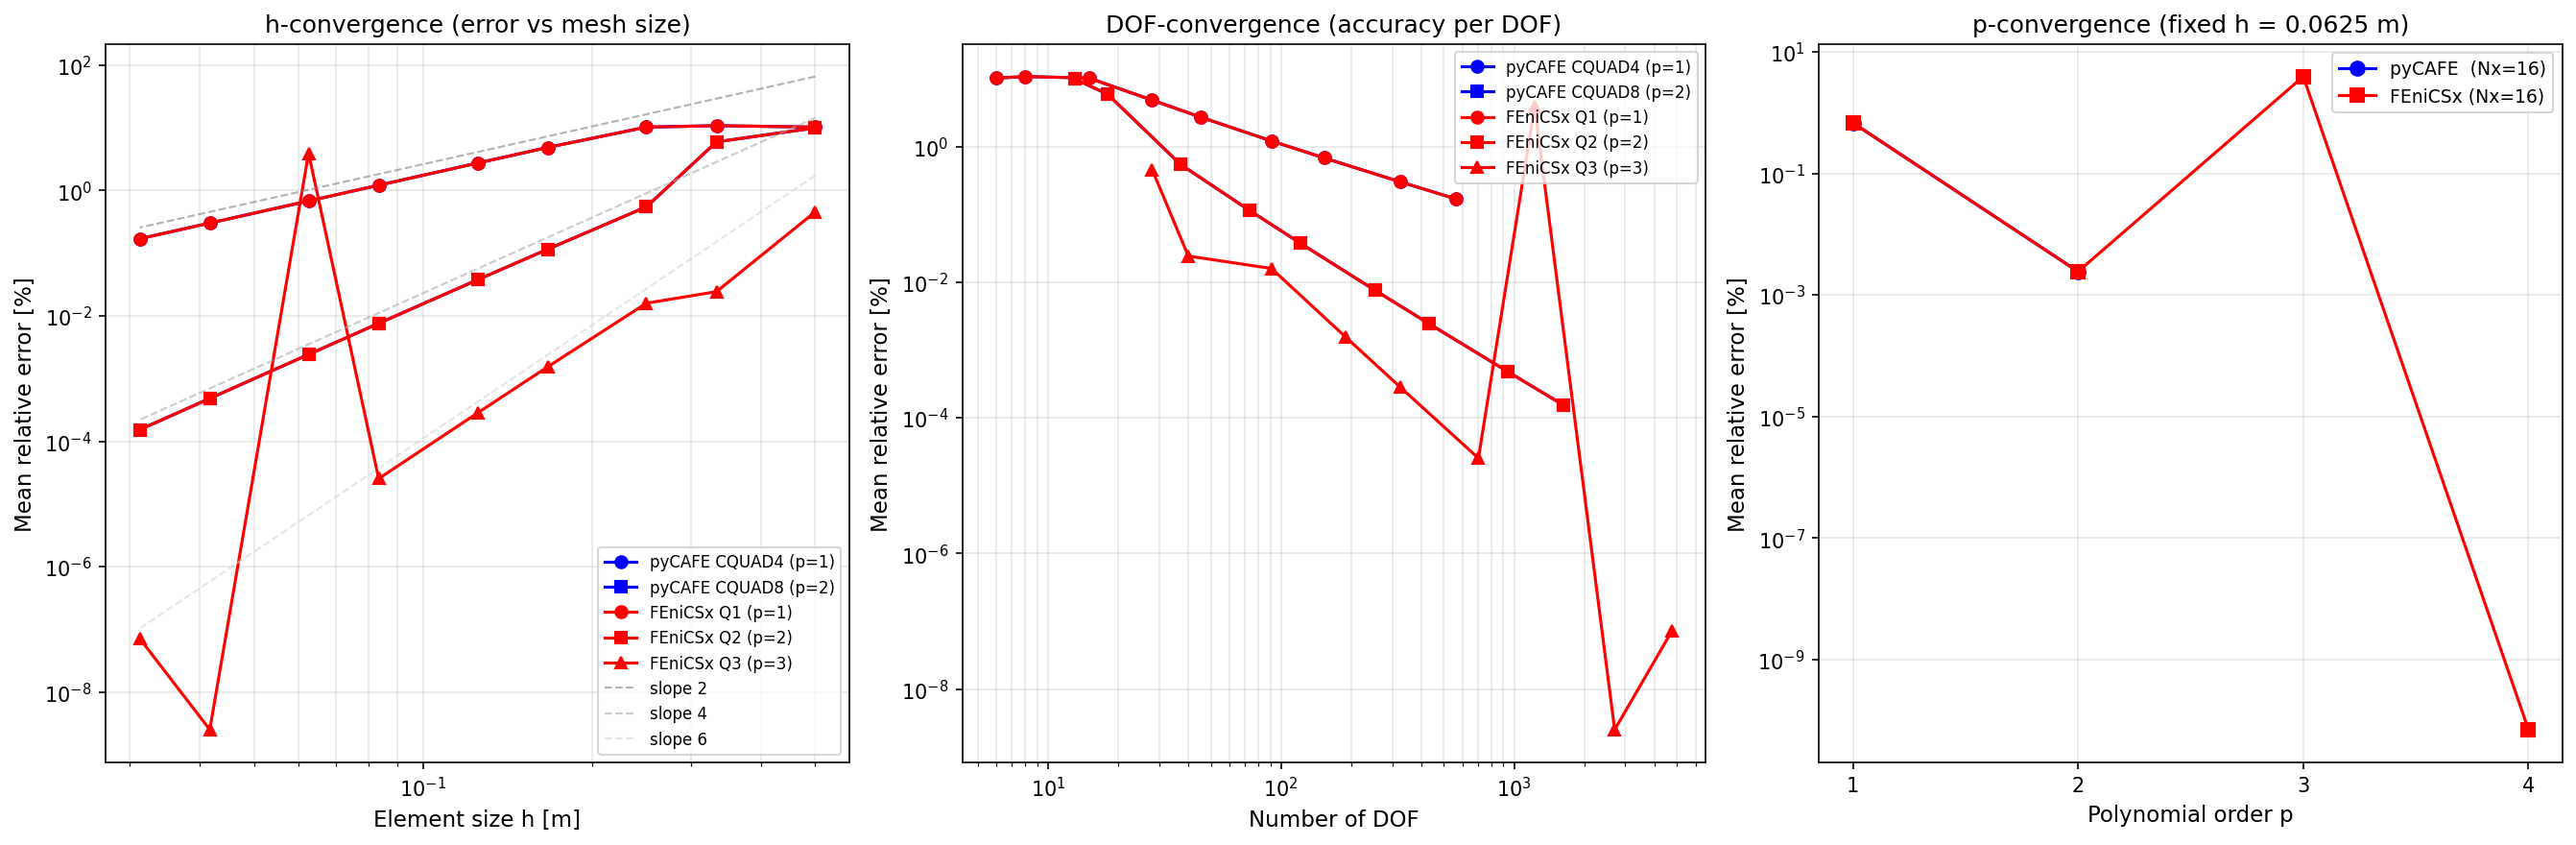
\includegraphics[width=0.8\linewidth]{examples/convergence_hp.png}
    \caption{Convergence of the first eigenfrequency relative error as a function of mesh refinement for CQUAD4 ($O(h^2)$) and CQUAD8 ($O(h^4)$) elements. Rigid rectangular cavity benchmark.}
    \label{Fig_conv}
\end{figure}

\subsection*{Comparison with FEniCSx}

An independent cross-validation against FEniCSx \cite{FEniCSx2023} has been performed for both the modal and the direct frequency-domain solvers, using Q2 (quadratic Lagrange quadrilateral) elements on the same rectangular cavity benchmark ($L_x = 1\,\text{m}$, $L_y = 0.5\,\text{m}$, air). Both solvers were run on identical meshes generated with Gmsh.

\textbf{Modal cross-validation.} The first 20 acoustic eigenfrequencies were computed with all-Neumann (rigid) boundary conditions on all walls. pyCAFE used CQUAD8 with 6\,337 DOFs; FEniCSx used Q2 Lagrange elements with 8\,385 DOFs. Figure~\ref{Fig_fenics_modal} shows the comparison: relative differences in eigenfrequencies are below $0.0001\,\%$ for all 20 modes, confirming that the assembled stiffness and mass matrices are consistent between the two independent implementations. Degenerate modes (same eigenvalue, different spatial orientation) are correctly resolved by both solvers. The full comparison is documented in notebook \texttt{examples/comparison\_pycafe\_fenics.ipynb}.

\begin{figure}[h]
    \centering
    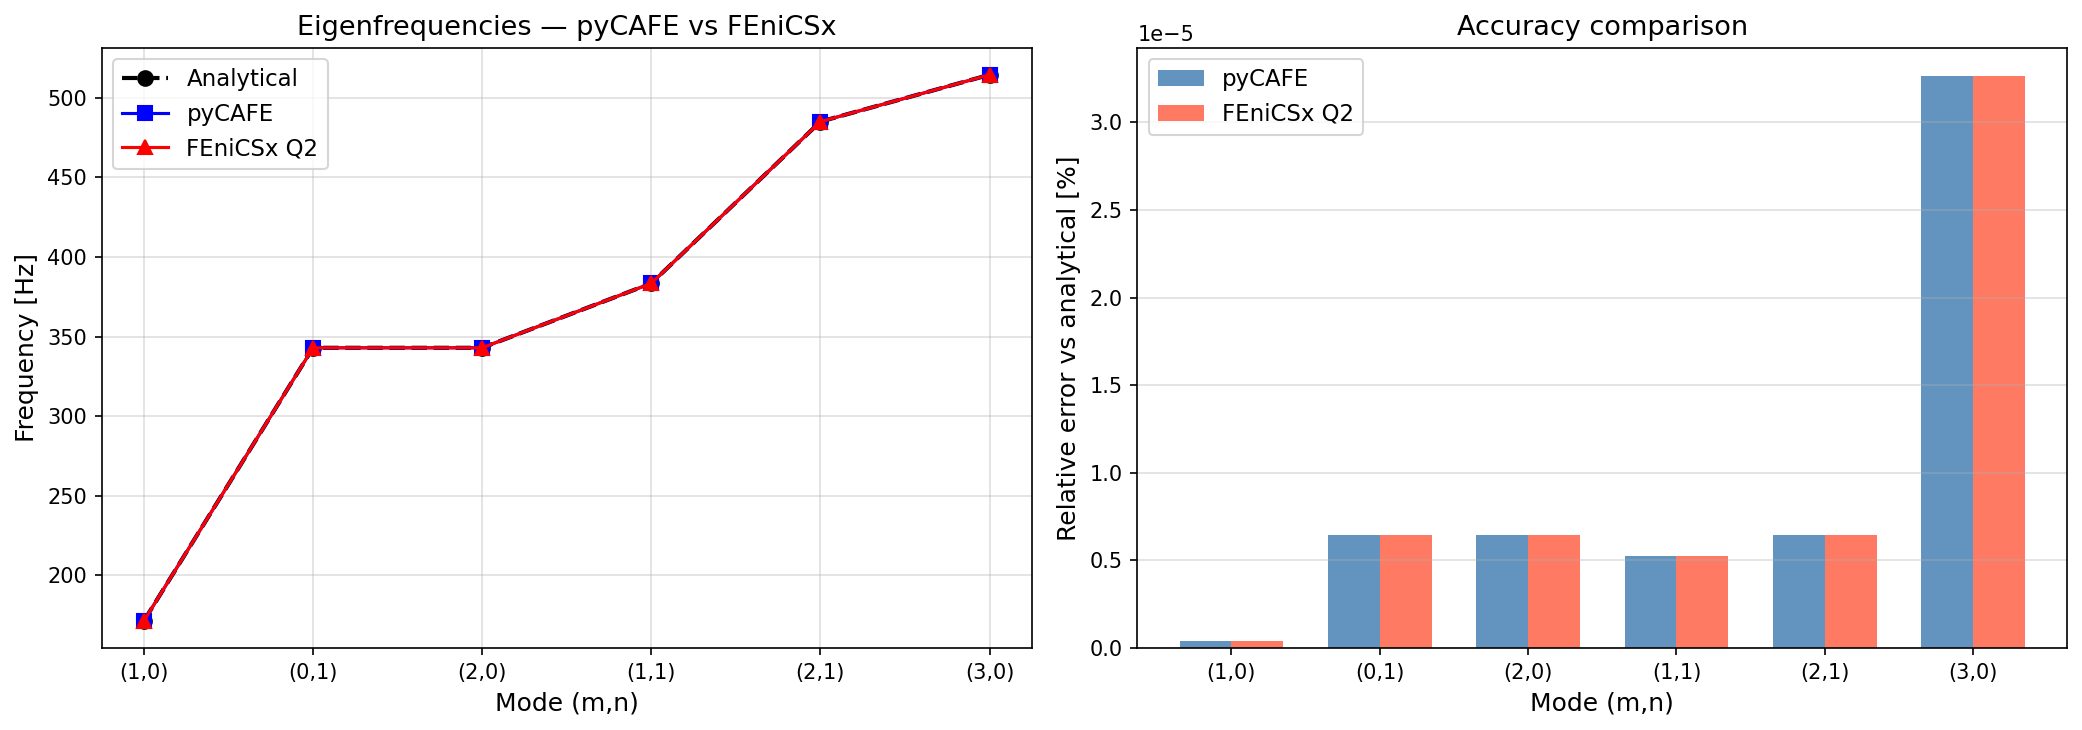
\includegraphics[width=0.8\linewidth]{examples/comparison_frequencies.png}
    \caption{Modal cross-validation: first 20 eigenfrequencies computed by pyCAFE (CQUAD8, 6\,337 DOFs) and FEniCSx (Q2, 8\,385 DOFs) on identical Gmsh meshes. Relative differences are below $0.0001\,\%$ for all modes.}
    \label{Fig_fenics_modal}
\end{figure}

\textbf{Direct frequency-domain (Helmholtz) cross-validation.} A systematic cross-validation of the direct solver was performed across four boundary condition configurations on the same rectangular cavity ($L_x = 1\,\text{m}$, $L_y = 0.5\,\text{m}$, air), each covering a frequency sweep from 50 to 800~Hz (151 equispaced points, step 5~Hz). pyCAFE (CQUAD8, 6\,337 DOFs) and FEniCSx (Q2, 8\,385 DOFs) were compared against each other and against the one-dimensional analytical solution for each configuration:

\begin{enumerate}
  \item \textbf{Piston / all rigid.} Uniform normal velocity $v_n = 1\,\text{m/s}$ on the left wall; rigid Neumann condition on the remaining walls. Probe at $(L_x, L_y/2)$. Analytical: $p = -\mathrm{i}\,\rho c_0 v_n / \sin(k L_x)$. Cross-error between pyCAFE and FEniCSx: median $0.0000\,\%$, max $0.0000\,\%$.
  \item \textbf{Prescribed pressure / all rigid.} Uniform pressure $p_0 = 1\,\text{Pa}$ imposed on the left wall (essential Dirichlet condition); rigid Neumann on all other walls. Probe at $(L_x, L_y/2)$. Analytical: $p = p_0 / \cos(k L_x)$. Cross-error: median $0.024\,\%$, max $0.56\,\%$. The small residual difference reflects the different mesh densities and is not a formulation discrepancy; both solvers agree with the analytical solution to within $0.03\,\%$ away from poles.
  \item \textbf{Piston / pressure-release right.} Normal velocity on the left wall; homogeneous Dirichlet ($p = 0$) on the right wall; rigid Neumann elsewhere. Probe at $(L_x/2, L_y/2)$. Analytical: $p = \mathrm{i}\,\rho c_0 v_n \sin(k(L_x - x)) / \cos(k L_x)$. Cross-error: median $0.067\,\%$, max $7.8\,\%$ (max occurs near poles of $\cos(kL_x)$ and is not a solver defect).
  \item \textbf{Piston / anechoic right.} Normal velocity on the left wall; perfectly absorbing impedance $Z = \rho c_0$ ($Z_\text{norm} = 1$) on the right wall. Probe at $(L_x/2, L_y/2)$. Analytical: $|p| = \rho c_0 v_n = \text{const}$ (no standing wave). Cross-error: median $0.0001\,\%$, max $0.0003\,\%$.
\end{enumerate}

Figure~\ref{Fig_fenics} shows the pressure magnitude, real part, and phase for all four cases. The pyCAFE (blue) and FEniCSx (red dashed) curves are visually indistinguishable and track the analytical reference (black dotted) throughout. Case~4 demonstrates that the impedance boundary condition correctly suppresses all standing-wave resonances: the pressure magnitude remains flat at $\approx413\,\text{Pa}$, the real part sweeps smoothly between $\pm\rho c_0 v_n$, and the phase advances linearly with frequency, consistent with a purely travelling wave.

\textbf{Equivalence of Dirichlet implementations.} A key aspect of the cross-validation is the comparison of how the two solvers handle prescribed pressure (essential) boundary conditions. In pyCAFE, zero-pressure conditions are enforced at assembly time by permanently deleting the corresponding rows and columns from the system matrices; non-zero prescribed pressures are handled at solve time via the partitioned system $\mathbf{A}_{ii}\,\mathbf{p}_i = \mathbf{f}_i - \mathbf{A}_{in}\,\mathbf{p}_0$ (static condensation, equation~(1)). In FEniCSx, the same static condensation is applied at solve time for all Dirichlet values. Both strategies are algebraically equivalent; the agreement in Cases~2 and~3 confirms that the two implementations are consistent. The full comparison is documented in \texttt{examples/test\_direct\_helmholtz\_pycafe\_fenics.py}.

\begin{figure}[h]
    \centering
    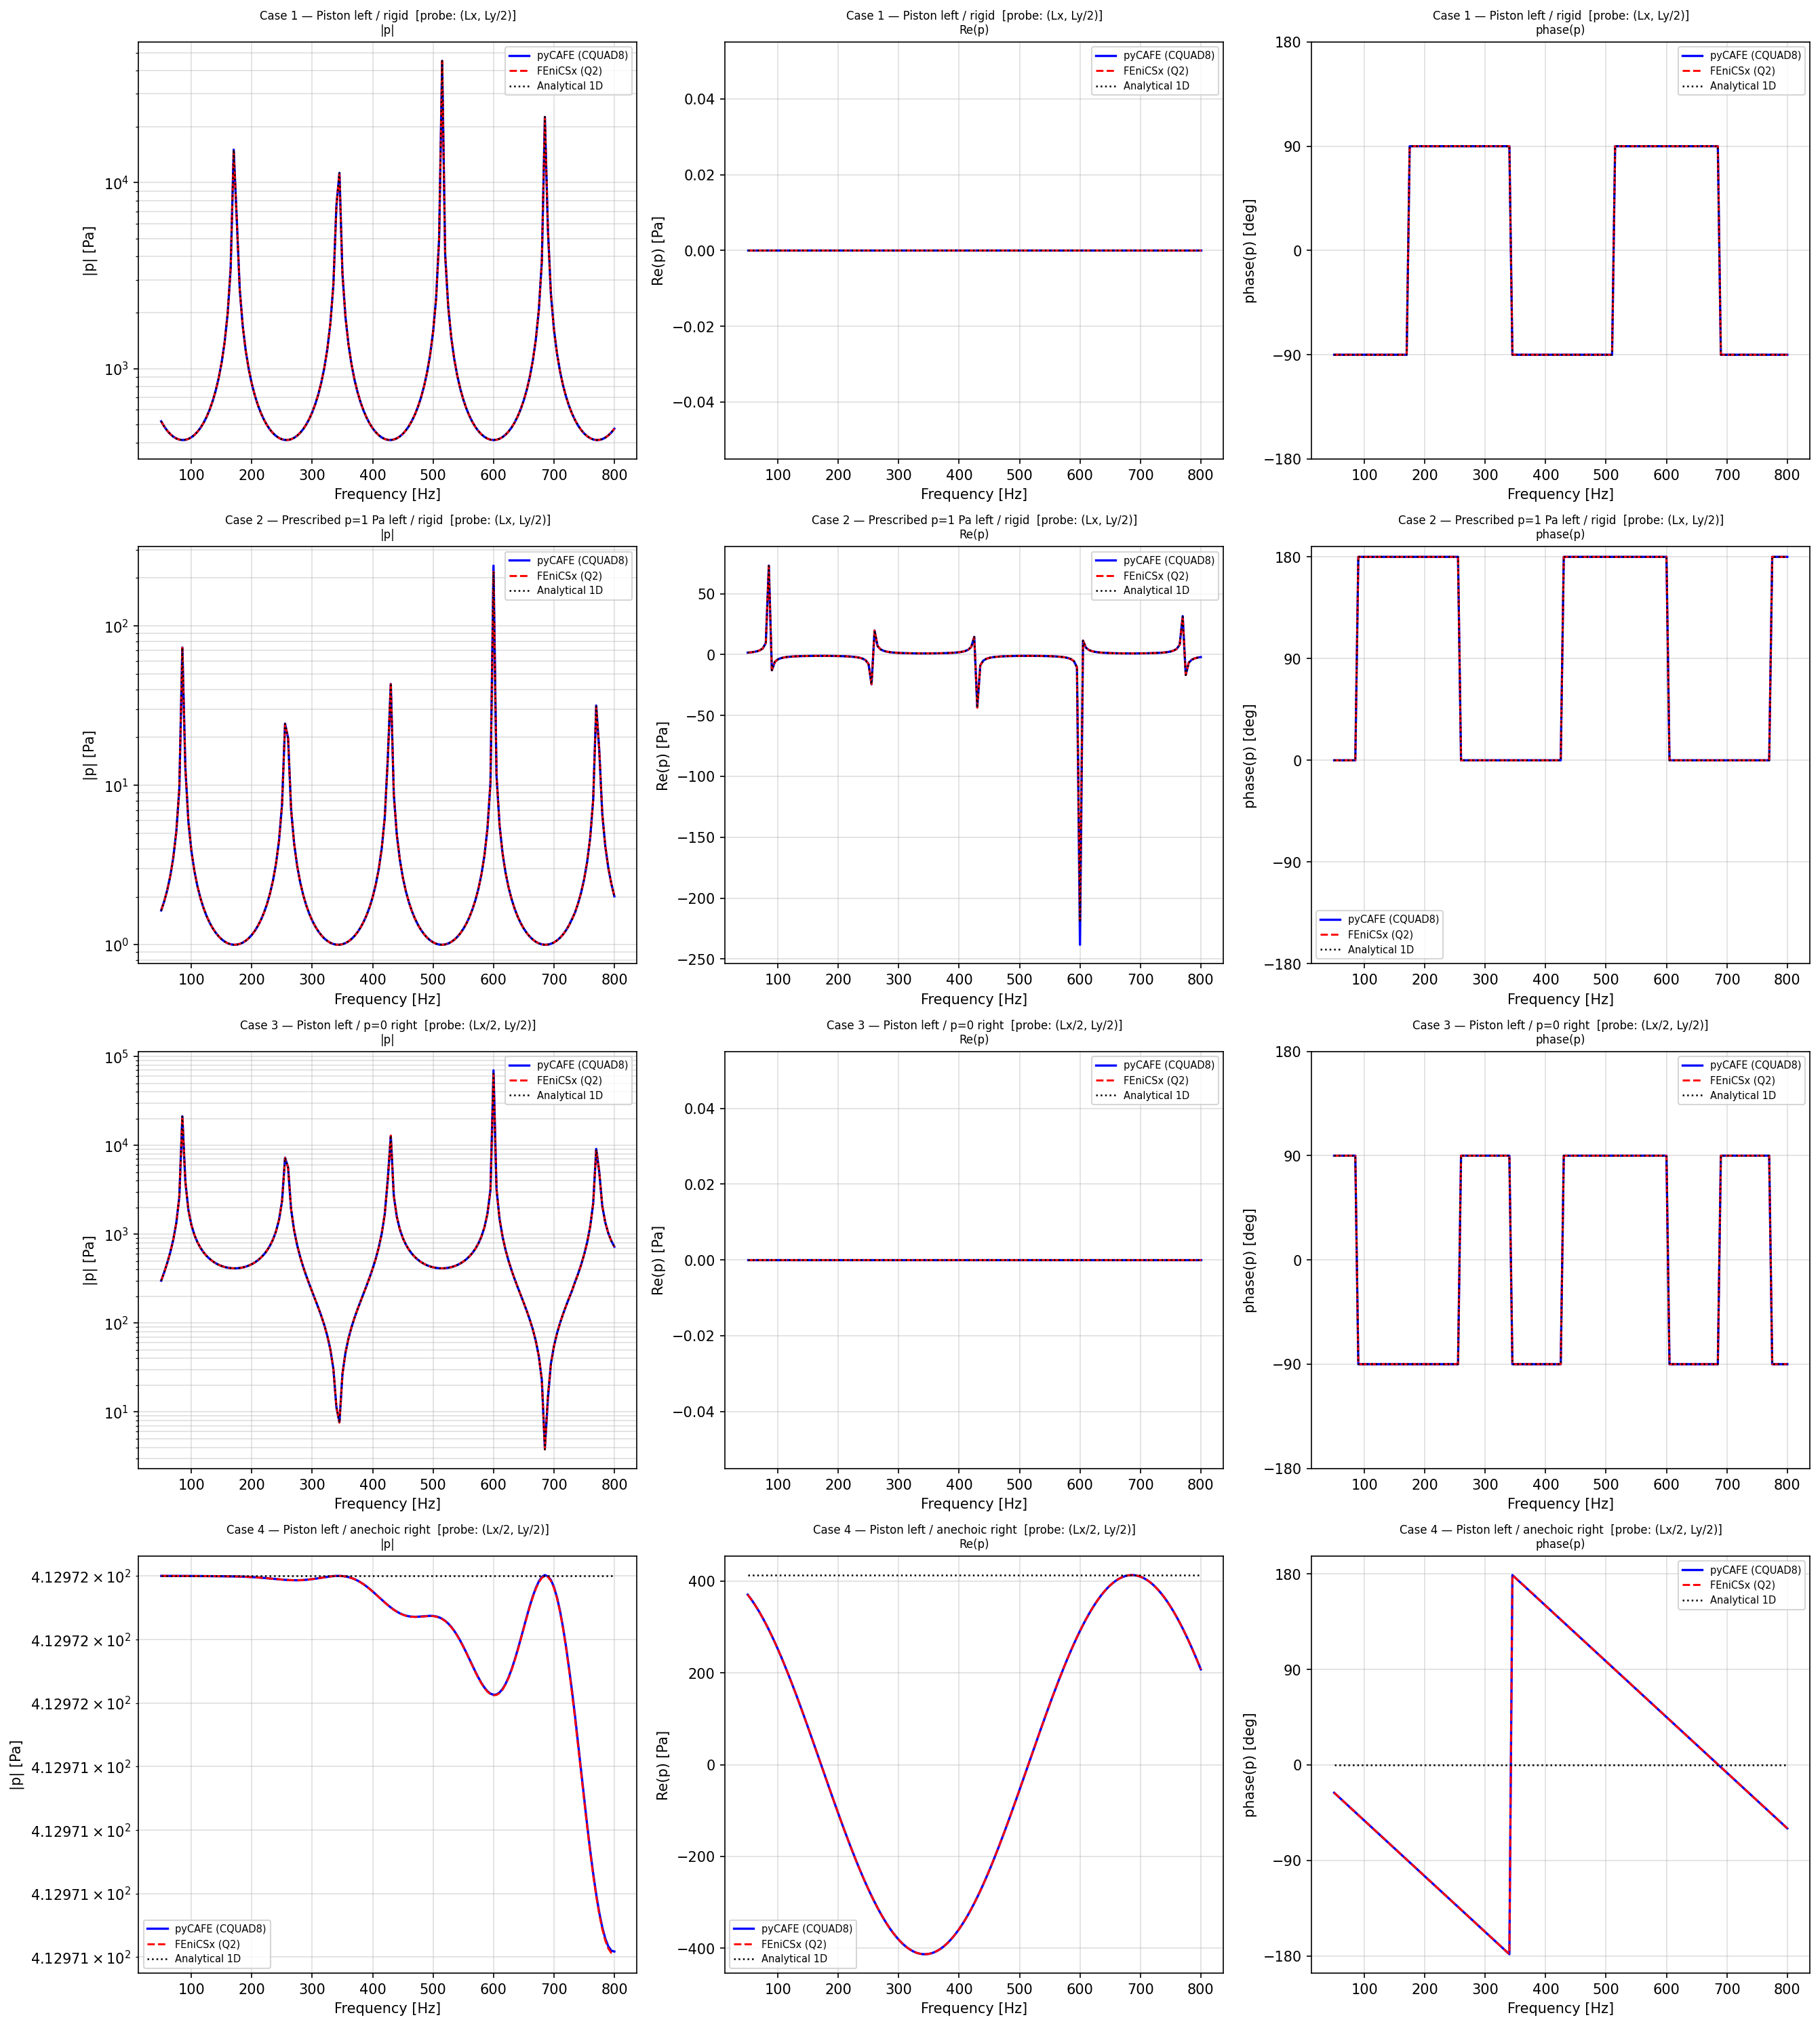
\includegraphics[width=\linewidth]{examples/test_direct_helmholtz_pycafe_fenics.png}
    \caption{Direct Helmholtz solver cross-validation (pyCAFE CQUAD8 vs FEniCSx Q2, 50--800~Hz): pressure magnitude $|p|$ (left column), real part $\mathrm{Re}(p)$ (centre), and phase (right column) at the probe point for four boundary condition configurations. Row~1: piston left / all rigid. Row~2: prescribed pressure left / all rigid. Row~3: piston left / pressure-release right. Row~4: piston left / anechoic right ($Z = \rho c_0$). Blue solid: pyCAFE; red dashed: FEniCSx; black dotted: 1D analytical.}
    \label{Fig_fenics}
\end{figure}

\subsection*{Comparison with commercial software}

In addition to the open-source cross-validation, the assembled system matrices have been assessed against [COMMERCIAL SOFTWARE NAME, VERSION]. Identical geometries, mesh discretisations, material properties, and boundary conditions were replicated; the resulting acoustic natural frequencies and mode shapes are compared in Figure~\ref{Fig2}. Agreement is within the expected numerical tolerance of the respective solvers.

\begin{figure}[h]
    \centering
    \includegraphics[width=0.8\linewidth]{2.jpg}
    \caption{Modal analysis results comparison between pyCAFE and [COMMERCIAL SOFTWARE NAME]. Geometry: rectangular cavity, rigid walls, air. Left: mode-shape contour plots. Right: natural frequency comparison.}
    \label{Fig2}
\end{figure}

\subsection*{Performance}

Typical two-dimensional acoustic problems with $\mathcal{O}(10^3)$ degrees of freedom solve in less than one second on consumer-grade hardware using the sparse direct solver. Modal analyses requesting the first $k$ modes with ARPACK scale as $O(N \cdot k)$, enabling problems with $\mathcal{O}(10^4)$ DOFs to be solved in a few seconds. Detailed DOF-versus-runtime data for the rectangular cavity benchmark are provided in the Jupyter notebooks \texttt{examples/convergence\_hp.ipynb} and \texttt{examples/pycafe\_convergence\_hp.ipynb}.


\section*{(2) Availability}
\vspace{0.5cm}
\section*{Operating system}

This package is compatible with macOS, Windows, and Linux operating systems supporting Python version 3.10 or newer. No operating system-specific features are required. Compatibility across Python 3.10, 3.11, and 3.12 is verified automatically via the GitHub Actions CI pipeline on every commit.

\section*{Programming language}
The software is implemented in Python (version $\geq 3.10$). All core functionalities, including mesh handling, matrix assembly, solvers, and post-processing utilities, are written in Python.

\section*{Additional system requirements}
No special hardware requirements are imposed. The software can be executed on standard desktop or laptop computers. Memory and CPU requirements scale with the size of the finite element model; typical two-dimensional acoustic problems with a few thousand degrees of freedom can be solved on consumer-grade hardware. The current implementation supports only two-dimensional geometries; three-dimensional extension is planned for future versions (see Section~Reuse~Potential). Input is provided via terminal-based interaction and external mesh files, while output consists of numerical data and optional graphical visualisations.

\section*{Dependencies}
The following Python packages are required for basic functionality:
\begin{itemize}
    \item \textbf{NumPy} ($\geq$ 1.20) \cite{Harris2020}: numerical arrays and vectorised operations
    \item \textbf{SciPy} ($\geq$ 1.8) \cite{Virtanen2020}: sparse linear algebra routines and frequency-domain solvers
    \item \textbf{Matplotlib} ($\geq$ 3.5) \cite{Hunter2007}: visualisation and post-processing of acoustic fields
    \item \textbf{tqdm} ($\geq$ 4.60): progress monitoring for frequency sweeps
    \item \textbf{Gmsh} ($\geq$ 4.10) \cite{Gmsh2009}: geometry definition and finite element mesh generation via the Python API
\end{itemize}
The package can be installed directly from PyPI:
\begin{verbatim}
pip install pycafe
\end{verbatim}

\section*{List of contributors}

\begin{itemize}
    \item \textbf{Daniele Fabbri}: conceptualisation, software development, numerical implementation, validation, and manuscript preparation.
    \item \textbf{Fabio Bruzzone}: scientific supervision, methodological guidance, and critical review of the numerical approach and software design.
    \item \textbf{Carlo Rosso}: scientific supervision, methodological guidance, and critical review of the numerical approach and software design.
\end{itemize}


\section*{Software location:}

{\bf Code repository} (GitHub)

\begin{description}[noitemsep,topsep=0pt]
	\item[Name:] pyCAFE
	\item[Persistent identifier:] \url{https://github.com/DanFabb/pycafe}
	\item[Licence:] MIT License
	\item[Date published:] 19/12/2025
\end{description}

{\bf Archived software version} (Zenodo)

\begin{description}[noitemsep,topsep=0pt]
	\item[Name:] pyCAFE
	\item[Persistent identifier:] \url{https://doi.org/[ZENODO DOI]}
	\item[Licence:] MIT License
	\item[Date published:] 15/04/2026
\end{description}

\section*{Language}
English

\section*{(3) Reuse potential}
The pyCAFE framework is designed to support acoustic investigations in two-dimensional domains discretised with quadrilateral finite elements, with a particular focus on low-to-mid frequency applications where FEM is most effective. Typical use cases include enclosed acoustic cavities, ducts, and generic 2D acoustic domains defined through externally generated meshes. The software supports both direct frequency-domain analyses and modal approaches, enabling its use for resonance studies, frequency sweeps, and validation benchmarks. pyCAFE is particularly suited for three overlapping use contexts: educational teaching, numerical benchmarking and cross-validation, and lightweight research simulation. The modular architecture facilitates reuse and extension; new finite elements, boundary conditions, or solver strategies can be incorporated by extending the corresponding submodules without modifying the core workflow.

\subsection*{Educational use}

The explicit matrix-based assembly and the keyboard-driven boundary condition interface make pyCAFE well suited for teaching finite element acoustics at graduate level. By exposing the global stiffness and mass matrices directly, students can inspect, modify, and validate the discretised operators, reinforcing the connection between the theoretical formulation and the numerical implementation. A step-by-step guided tutorial notebook (\texttt{examples/analisi\_modale\_guidata.ipynb}) walks through a complete modal analysis workflow: fluid selection (air or water), mesh loading, boundary condition assignment (rigid walls, pressure-release boundaries), eigenfrequency computation, and mode-shape visualisation. The tutorial includes guided experiments on the effect of boundary condition type on resonance frequencies, directly comparing computed results against the analytical closed-form solution, making it appropriate for both self-study and structured laboratory sessions.

\subsection*{Benchmarking and cross-validation}

The transparent matrix-based design makes pyCAFE a convenient lightweight reference implementation for benchmarking purposes. The explicitly assembled stiffness and mass matrices can be extracted, inspected, and compared against independent implementations at the operator level. Two independent cross-validation paths are provided and documented:
\begin{itemize}
    \item \textbf{Analytical}: eigenfrequencies of a rigid rectangular cavity compared against the closed-form solution (Table~\ref{tab:validation}; relative errors $< 0.001\,\%$ with CQUAD8).
    \item \textbf{FEniCSx Q2}: both modal eigenfrequencies (Figure~\ref{Fig_fenics_modal}; differences $< 0.0001\,\%$ for 20 modes) and direct Helmholtz frequency response functions (Figure~\ref{Fig_fenics}; median error $< 0.001\,\%$ across a 50--800~Hz sweep) are validated against FEniCSx.
\end{itemize}
These benchmarks cover both solver paths (eigenvalue and direct) and both boundary condition types (all-Neumann and mixed velocity/rigid), providing a comprehensive validation baseline. The same framework can be used to verify new element formulations or boundary condition implementations by adding the corresponding element module and running the existing test suite.

\subsection*{Research simulation}

For research applications, pyCAFE provides a self-contained Python workflow for parametric frequency-domain acoustic studies. The direct solver supports single-frequency analyses and broadband frequency sweeps with impedance, velocity, or pressure boundary conditions. The modal solver provides natural frequencies and mode shapes that can be used as a reduced-order basis for efficient parametric studies \cite{Cai2024}. An example of a general interactive simulation workflow, including mesh loading, boundary condition assignment, and post-processing of the acoustic pressure field, is demonstrated in \texttt{examples/Example1.ipynb}. Figure~\ref{Fig3} shows a representative graphical output from a frequency sweep simulation.

\begin{figure}[h]
    \centering
    \includegraphics[width=0.8\linewidth]{3.jpg}
    \caption{Graphical output of a frequency sweep simulation using pyCAFE: acoustic pressure field reconstructed over the 2D computational domain.}
    \label{Fig3}
\end{figure}

\subsection*{Future work}

Planned extensions beyond version 1.0.0 are summarised in Figure~\ref{Fig4} and include:
\begin{itemize}
    \item \textbf{Three-dimensional elements}: extension to hexahedral (HEX8, HEX20) and tetrahedral elements to support 3D acoustic cavities and enclosures.
    \item \textbf{Perfectly Matched Layers (PML)}: implementation of PML absorbing regions for simulation of unbounded domains and radiation problems in 2D \cite{Beriot2021,Turkel1998}.
    \item \textbf{Time-domain solver}: addition of explicit and implicit time-integration schemes for transient acoustic problems.
    \item \textbf{Vibroacoustic coupling}: structural--acoustic coupling by assembling a combined structural--fluid system using the existing matrix-based framework \cite{Nefske1976}.
    \item \textbf{Extended post-processing}: sound power computation, directivity maps, and export to standard data formats.
    \item \textbf{Conda distribution}: the package is available on PyPI (\texttt{pip install pycafe}); a Conda package is planned.
\end{itemize}

Contributions from the community are encouraged, and users interested in extending the software are invited to open an issue or pull request on the public code repository.

\begin{figure}[h]
    \centering
    \includegraphics[width=0.8\linewidth]{4.jpg}
    \caption{Roadmap for future pyCAFE versions.}
    \label{Fig4}
\end{figure}


\section*{Funding statement}
This publication is part of the project PNRR-NGEU which has received funding from the MUR -- DM 117/2023.
\

\begin{thebibliography}{99}

\bibitem{MacNeal1994}
MacNeal, R. H. (1994).
\textit{Finite Elements: Their Design and Performance}.
New York, NY: Marcel Dekker.

\bibitem{Desmet1999}
Desmet, W. and Vandepitte, D. (1999).
Finite element method in acoustics.
\textit{Proceedings of ISMA 1999}, Leuven, Belgium.

\bibitem{Ihlenburg1995}
Ihlenburg, F. and Babu{\v{s}}ka, I. (1995).
Finite element solution of the Helmholtz equation with high wave number.
Part I: The h-version of the FEM.
\textit{Computers \& Mathematics with Applications}, 30(9), pp. 9--37.\\
DOI: \url{https://doi.org/10.1016/0898-1221(95)00144-N}

\bibitem{Babuska1988}
Babu{\v{s}}ka, I. (1988).
The p and h-p versions of the finite element method: The state of the art.
In: Dwoyer, D. L., Hussaini, M. Y. and Voigt, R. G. (eds.),
\textit{Finite Elements}.
New York, NY: Springer, pp. 199--239.\\
DOI: \url{https://doi.org/10.1007/978-1-4612-3786-0_10}

\bibitem{Prinn2023}
Prinn, A. G. (2023).
A review of finite element methods for room acoustics.
\textit{Acoustics}, 5(2), pp. 367--395.\\
DOI: \url{https://doi.org/10.3390/acoustics5020022}

\bibitem{HelmholtzResonator2012}
Cosma, I. A., Maier, V. and Mihon, L. (2012).
Considerations on the Helmholtz resonator simulation and experiment.
\textit{Proceedings of the Romanian Academy Series A -- Mathematics, Physics, Technical Sciences, Information Science},
vol. 13, no. 2, pp. 141--148.

\bibitem{Thompson2006}
Thompson, L. L. (2006).
A review of finite-element methods for time-harmonic acoustics.
\textit{The Journal of the Acoustical Society of America}, 119(3), pp. 1315--1330.\\
DOI: \url{https://doi.org/10.1121/1.2164987}

\bibitem{Harari2006}
Harari, I. (2006).
A survey of finite element methods for time-harmonic acoustics.
\textit{Computer Methods in Applied Mechanics and Engineering}, 195(13), pp. 1594--1607.\\
DOI: \url{https://doi.org/10.1016/j.cma.2005.05.030}

\bibitem{Khalefa2024}
Khalefa, S. J. (2024).
An analytic and numerical study of Helmholtz equation using finite element method.
\textit{Mathematical Modelling of Engineering Problems}, 11(12), pp. 3440--3446.\\
DOI: \url{https://doi.org/10.18280/mmep.111222}

\bibitem{Nefske1976}
Wolf, J. A., Nefske, D. J. and Howell, L. J. (1976).
Structural--Acoustic Finite Element Analysis of the Automobile Passenger Compartment.
\textit{1976 Automotive Engineering Congress and Exposition}.
SAE International.\\
DOI: \url{https://doi.org/10.4271/760184}

\bibitem{Beriot2021}
B\'{e}riot, H. and Modave, A. (2021).
An automatic perfectly matched layer for acoustic finite element simulations in convex domains of general shape.
\textit{International Journal for Numerical Methods in Engineering}, 122(5), pp. 1239--1261.\\
DOI: \url{https://doi.org/10.1002/nme.6560}

\bibitem{Turkel1998}
Turkel, E. and Yefet, A. (1998).
Absorbing PML boundary layers for wave-like equations.
\textit{Applied Numerical Mathematics}, 27(4), pp. 533--557.\\
DOI: \url{https://doi.org/10.1016/S0168-9274(98)00026-9}

\bibitem{Pekel1995}
Pekel, U. and Mittra, R. (1995).
An application of the perfectly matched layer (PML) concept to the finite element method frequency-domain analysis of scattering problems.
\textit{IEEE Microwave and Guided Wave Letters}, 5(8), pp. 258--260.\\
DOI: \url{https://doi.org/10.1109/75.401074}

\bibitem{Reheman2013}
Reheman, P. and Shiojiri, H. (2013).
Application of PML to analysis of nonlinear soil--structure--fluid problems using mixed elements.
\textit{International Journal of GEOMATE}, 4, pp. 505--510.\\
DOI: \url{https://doi.org/10.21660/2013.8.2167}

\bibitem{Fabbri2025}
Fabbri, D., Bruzzone, F. and Rosso, C. (2025).
Acoustic field solution in a pipe using CAFE.
\textit{Proceedings of the OpenSD 2025 Conference}, Ljubljana, Slovenia, 16--17 June 2025.
University of Ljubljana, Faculty of Mechanical Engineering, pp.~48--51.
ISBN: 978-961-7187-17-5.

\bibitem{Gmsh2009}
Geuzaine, C. and Remacle, J.-F. (2009).
Gmsh: A 3-D finite element mesh generator with built-in pre- and post-processing facilities.
\textit{International Journal for Numerical Methods in Engineering}, 79(11), pp. 1309--1331.\\
DOI: \url{https://doi.org/10.1002/nme.2579}

\bibitem{Beriot2016}
B\'{e}riot, H., Prinn, A. and Gabard, G. (2016).
Efficient implementation of high-order finite elements for Helmholtz problems.
\textit{International Journal for Numerical Methods in Engineering}, 106(3), pp. 213--240.\\
DOI: \url{https://doi.org/10.1002/nme.5172}

\bibitem{Guyan1965}
Guyan, R. J. (1965).
Reduction of stiffness and mass matrices.
\textit{AIAA Journal}, 3(2), p. 380.\\
DOI: \url{https://doi.org/10.2514/3.2874}

\bibitem{Kidder1973}
Kidder, R. L. (1973).
Reduction of structural frequency equations.
\textit{AIAA Journal}, 11(6), p. 892.\\
DOI: \url{https://doi.org/10.2514/3.6852}

\bibitem{Cai2024}
Cai, Y., van Ophem, S., Wu, S., Desmet, W. and Deckers, E. (2024).
Model order reduction of time-domain acoustic finite element simulations with perfectly matched layers.
\textit{Computer Methods in Applied Mechanics and Engineering}, 431, 117298.\\
DOI: \url{https://doi.org/10.1016/j.cma.2024.117298}

\bibitem{Damhaug1993}
Damhaug, A. C., Mathisen, K. M. and Okstad, K. M. (1993).
The use of sparse matrix methods in finite-element codes for structural mechanics applications.
\textit{Computing Systems in Engineering}, 4(4), pp.~355--362.\\
DOI: \url{https://doi.org/10.1016/0956-0521(93)90003-F}

\bibitem{Harris2020}
Harris, C. R., Millman, K. J., van der Walt, S. J., Gommers, R., Virtanen, P.,
Cournapeau, D., Wieser, E., Taylor, J., Berg, S., Smith, N. J., Kern, R.,
Picus, M., Hoyer, S., van Kerkwijk, M. H., Brett, M., Haldane, A.,
Fern{\'a}ndez del R{\'i}o, J., Wiebe, M., Peterson, P., G{\'e}rard-Marchant, P.,
Sheppard, K., Reddy, T., Weckesser, W., Abbasi, H., Gohlke, C. and Oliphant, T. E. (2020).
Array programming with NumPy.
\textit{Nature}, 585(7825), pp.~357--362.\\
DOI: \url{https://doi.org/10.1038/s41586-020-2649-2}

\bibitem{Virtanen2020}
Virtanen, P., Gommers, R., Oliphant, T. E., Haberland, M., Reddy, T.,
Cournapeau, D., Burovski, E., Peterson, P., Weckesser, W., Bright, J.,
van der Walt, S. J., Brett, M., Wilson, J., Millman, K. J., Mayorov, N.,
Nelson, A. R. J., Jones, E., Kern, R., Larson, E., Carey, C. J.,
Polat, {\.I}., Feng, Y., Moore, E. W., VanderPlas, J., Laxalde, D.,
Perktold, J., Cimrman, R., Henriksen, I., Quintero, E. A., Harris, C. R.,
Archibald, A. M., Ribeiro, A. H., Pedregosa, F., van Mulbregt, P. and
SciPy 1.0 Contributors (2020).
SciPy 1.0: Fundamental algorithms for scientific computing in Python.
\textit{Nature Methods}, 17, pp.~261--272.\\
DOI: \url{https://doi.org/10.1038/s41592-019-0686-2}

\bibitem{Hunter2007}
Hunter, J. D. (2007).
Matplotlib: A 2D graphics environment.
\textit{Computing in Science \& Engineering}, 9(3), pp.~90--95.\\
DOI: \url{https://doi.org/10.1109/MCSE.2007.55}

\bibitem{FEniCSx2023}
Baratta, I. A., Dean, J. P., Dokken, J. S., Habera, M., Hale, J. S.,
Richardson, C. N., Rognes, M. E., Scroggs, M. W., Sime, N. and Wells, G. N. (2023).
DOLFINx: The next generation FEniCS problem solving environment.
\textit{Zenodo}.\\
DOI: \url{https://doi.org/10.5281/zenodo.10447666}

\bibitem{Hecht2012}
Hecht, F. (2012).
New development in FreeFem++.
\textit{Journal of Numerical Mathematics}, 20(3-4), pp. 251--265.\\
DOI: \url{https://doi.org/10.1515/jnum-2012-0013}

\bibitem{skfem2020}
Gustafsson, T. and McBain, G. D. (2020).
scikit-fem: A Python package for finite element assembly.
\textit{Journal of Open Source Software}, 5(52), 2369.\\
DOI: \url{https://doi.org/10.21105/joss.02369}

\bibitem{openCFS2022}
Kaltenbacher, M., Floss, S., Toth, F. and Kaltenbacher, B. (2022).
openCFS: Open source finite element software for coupled field simulation.
\textit{SoftwareX}, 20, 101267.\\
DOI: \url{https://doi.org/10.1016/j.softx.2022.101267}

\end{thebibliography}

{ \bf Copyright Notice} \\
Authors who publish with this journal agree to the following terms: \\

Authors retain copyright and grant the journal right of first publication with the work simultaneously licensed under a  \href{http://creativecommons.org/licenses/by/3.0/}{Creative Commons Attribution License} that allows others to share the work with an acknowledgement of the work's authorship and initial publication in this journal. \\

Authors are able to enter into separate, additional contractual arrangements for the non-exclusive distribution of the journal's published version of the work (e.g., post it to an institutional repository or publish it in a book), with an acknowledgement of its initial publication in this journal. \\

By submitting this paper you agree to the terms of this Copyright Notice, which will apply to this submission if and when it is published by this journal.


\end{document}
